\documentclass{beamer}
\usepackage[UKenglish]{babel}
\usepackage[UKenglish]{isodate}
\usepackage{adjustbox}
\usepackage{graphicx}
\usepackage[binary-units=true]{siunitx}
\usepackage{tikz}
\usepackage{tikz-uml}

\usetikzlibrary{arrows.meta}
\usetheme{Boadilla}
\usecolortheme{seahorse}
\beamertemplatenavigationsymbolsempty

\author{Paulius Dilkas}
\title[Automated Benchmarking]{Automated Benchmarking of Container Applications}
\date{1st August 2019}

\begin{document}

\maketitle

\begin{frame}{Main Ingredients}
  \centering
  
\includegraphics[height=0.89\textheight]{creation.jpg}
  \begin{tikzpicture}[remember picture,overlay]
    \node at (-7.5, 4.5) {
\includegraphics[width=100pt]{openshift.png}};
    \node at (-2.6, 5) {\colorbox{white}{
\includegraphics[width=50pt]{docker.png}}};
    \node at (-7.5, 0.9) {
\includegraphics[width=75pt]{flink.png}};
    \node at (-2.6, 0.7) {\colorbox{white}{
\includegraphics[width=100pt]{prometheus.png}}};
  \end{tikzpicture}
\end{frame}

\begin{frame}{The General Idea}
  \centering
  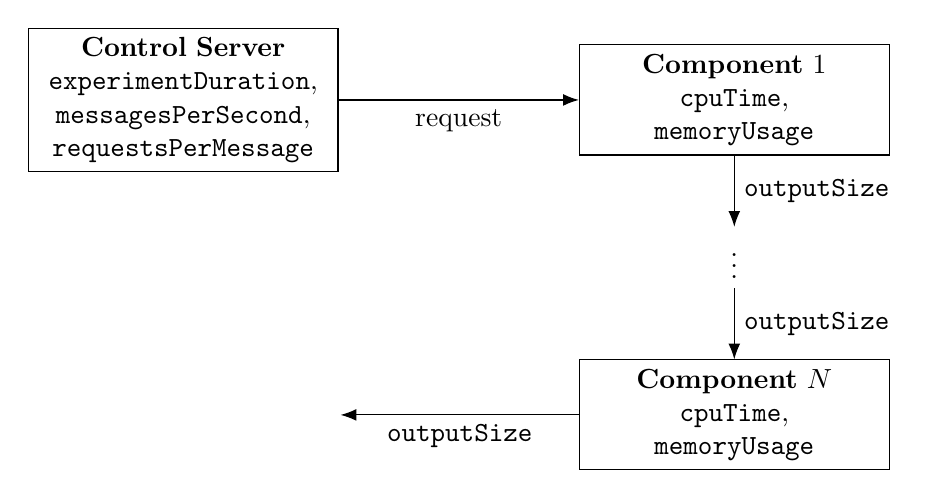
\begin{tikzpicture}[component/.style={draw, text width=3.7cm, align=center}]
    \node[component] at (-1, 0) (server) {
      \textbf{Control Server}\\
      \texttt{experimentDuration},\\
      \texttt{messagesPerSecond},\\
      \texttt{requestsPerMessage}
    };
    \node[component] at (6, 0) (component1) {
      \textbf{Component $1$}\\
      \texttt{cpuTime},\\
      \texttt{memoryUsage}
    };
    \node at (6, -2) (dotdotdot) {$\vdots$};
    \node[component] at (6, -4) (componentn) {
      \textbf{Component $N$}\\
      \texttt{cpuTime},\\
      \texttt{memoryUsage}
    };
    \draw[-{Latex[length=2mm]}] (server) -- node[below] {request} (component1);
    \draw[-{Latex[length=2mm]}] (component1) -- node[right] {\texttt{outputSize}} (dotdotdot);
    \draw[-{Latex[length=2mm]}] (dotdotdot) -- node[right] {\texttt{outputSize}} (componentn);
    \draw[-{Latex[length=2mm]}] (componentn) -- node[below] {\texttt{outputSize}} (1, -4);
  \end{tikzpicture}
\end{frame}

% \begin{frame}{Deployment}
%   \begin{adjustbox}{max totalsize={\textwidth}{0.88\textheight},center}
%     \begin{tikzpicture}
%       % components: first column
%       \umlbasiccomponent[x=-6, y=3, fill=cyan!20]{Prometheus}
%       \begin{umlcomponent}[fill=cyan!20]{Configuration Files}
%         \umlbasiccomponent[x=-6, y=-2, fill=red!20]{Global}
%         \umlbasiccomponent[x=-6, y=-4, fill=red!20]{Components}
%       \end{umlcomponent}

%       % components: second column
%       \umlbasiccomponent[x=0, y=1]{Control Service}
%       \begin{umlcomponent}{Control Pod}
%         \umlbasiccomponent[x=0, y=-2, fill=red!20]{Control Server}
%         \umlbasiccomponent[x=0, y=-4, fill=red!20]{Benchmarker}
%       \end{umlcomponent}
%       \umlbasiccomponent[x=0, y=-7]{Control Persistent Volume Claim}
%       \umlbasiccomponent[x=0, y=-10]{Control Persistent Volume}

%       % components: third column
%       \umlbasiccomponent[x=6, y=3]{JobManager Service}
%       \umlbasiccomponent[x=6, y=-1]{JobManager Pod}
%       \umlbasiccomponent[x=6, y=-4]{TaskManager Service}
%       \umlbasiccomponent[x=6, y=-8]{TaskManager Pod}

%       % connections in second column
%       \umlVHVassemblyconnector{Control Persistent Volume Claim}{Control Persistent Volume}
%       \umlVHVassemblyconnector{Control Pod}{Control Persistent Volume Claim}
%       \umlprovidedinterface[interface=998, with port, distance=2.5]{Control Server}
%       \umlrequiredinterface[interface=998, with port]{Benchmarker}
%       \umlHVassemblyconnector{Control Service}{Control Server-west-interface}
%       \umlHVassemblyconnector{Control Service}{Benchmarker-east-interface}

%       % connections between first and second columns
%       \umlHVHassemblyconnector[interface={\space}, arm1=-2.3]{Benchmarker}{Global}
%       \umlVHVassemblyconnector[interface={\space}]{Control Server}{Global}
%       \umlVHVassemblyconnector[interface={\space}, arm1=-0.7]{Benchmarker}{Components}

%       % Prometheus connections
%       \umlHVHassemblyconnector[interface=HTTPS, arm1=-2, with port]{Control Server}{Prometheus}
%       \umlassemblyconnector[interface=9250, arm1=1, with port]{Prometheus}{JobManager Service}
%       \umlHVHassemblyconnector[interface=9250, arm1=8, with port]{Prometheus}{TaskManager Service}

%       % column 3 connections
%       \umlVHVassemblyconnector[interface={6123{,} 6124{,} 8081{,} 9250}, with port]{JobManager Pod}{JobManager Service}
%       \umlVHVassemblyconnector[interface={6121{,} 6122{,} 9250}, with port]{TaskManager Pod}{TaskManager Service}
%     \end{tikzpicture}
%   \end{adjustbox}
% \end{frame}

\begin{frame}{Execution}
  \begin{adjustbox}{max totalsize={\textwidth}{\textheight},center}
    \begin{tikzpicture}
      \begin{umlseqdiag}
        \umlobject[no ddots]{Benchmarker}
        \umlobject[no ddots]{ControlServer}
        \umlobject[no ddots]{Prometheus}
        \umldatabase[no ddots]{PersistentVolume}
        \begin{umlcall}[op={initialise stream}]{Benchmarker}{ControlServer}
          \begin{umlfragment}[type=loop, label={$\forall$ messages}, inner xsep=7]
            \begin{umlcall}[op={message}, type=return]{ControlServer}{Benchmarker}
            \end{umlcall}
          \end{umlfragment}
        \end{umlcall}
        \begin{umlcall}[op={runtime}, type=return]{Benchmarker}{ControlServer}
        \end{umlcall}
        \begin{umlfragment}[type=loop, label={$\forall$ metrics}, inner xsep=6]
          \begin{umlcall}[op={query}, return={metric}]{ControlServer}{Prometheus}
          \end{umlcall}
          \begin{umlcall}[op={metric}]{ControlServer}{PersistentVolume}
          \end{umlcall}
        \end{umlfragment}
      \end{umlseqdiag}
    \end{tikzpicture}
  \end{adjustbox}
\end{frame}

\begin{frame}{Calibration}
  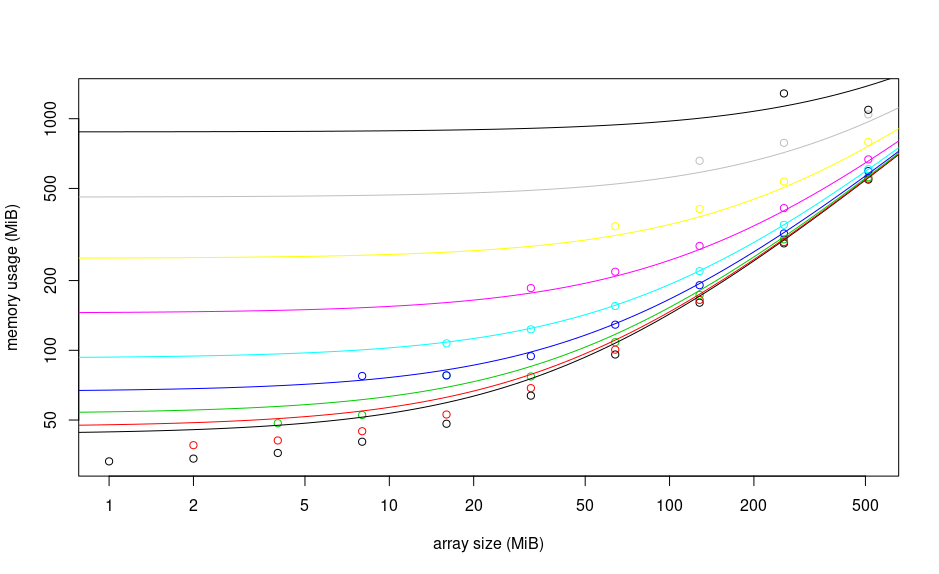
\includegraphics[width=\textwidth]{../../proof_of_concept/prediction1.png}
\end{frame}

\begin{frame}{Evaluation: CPU}
  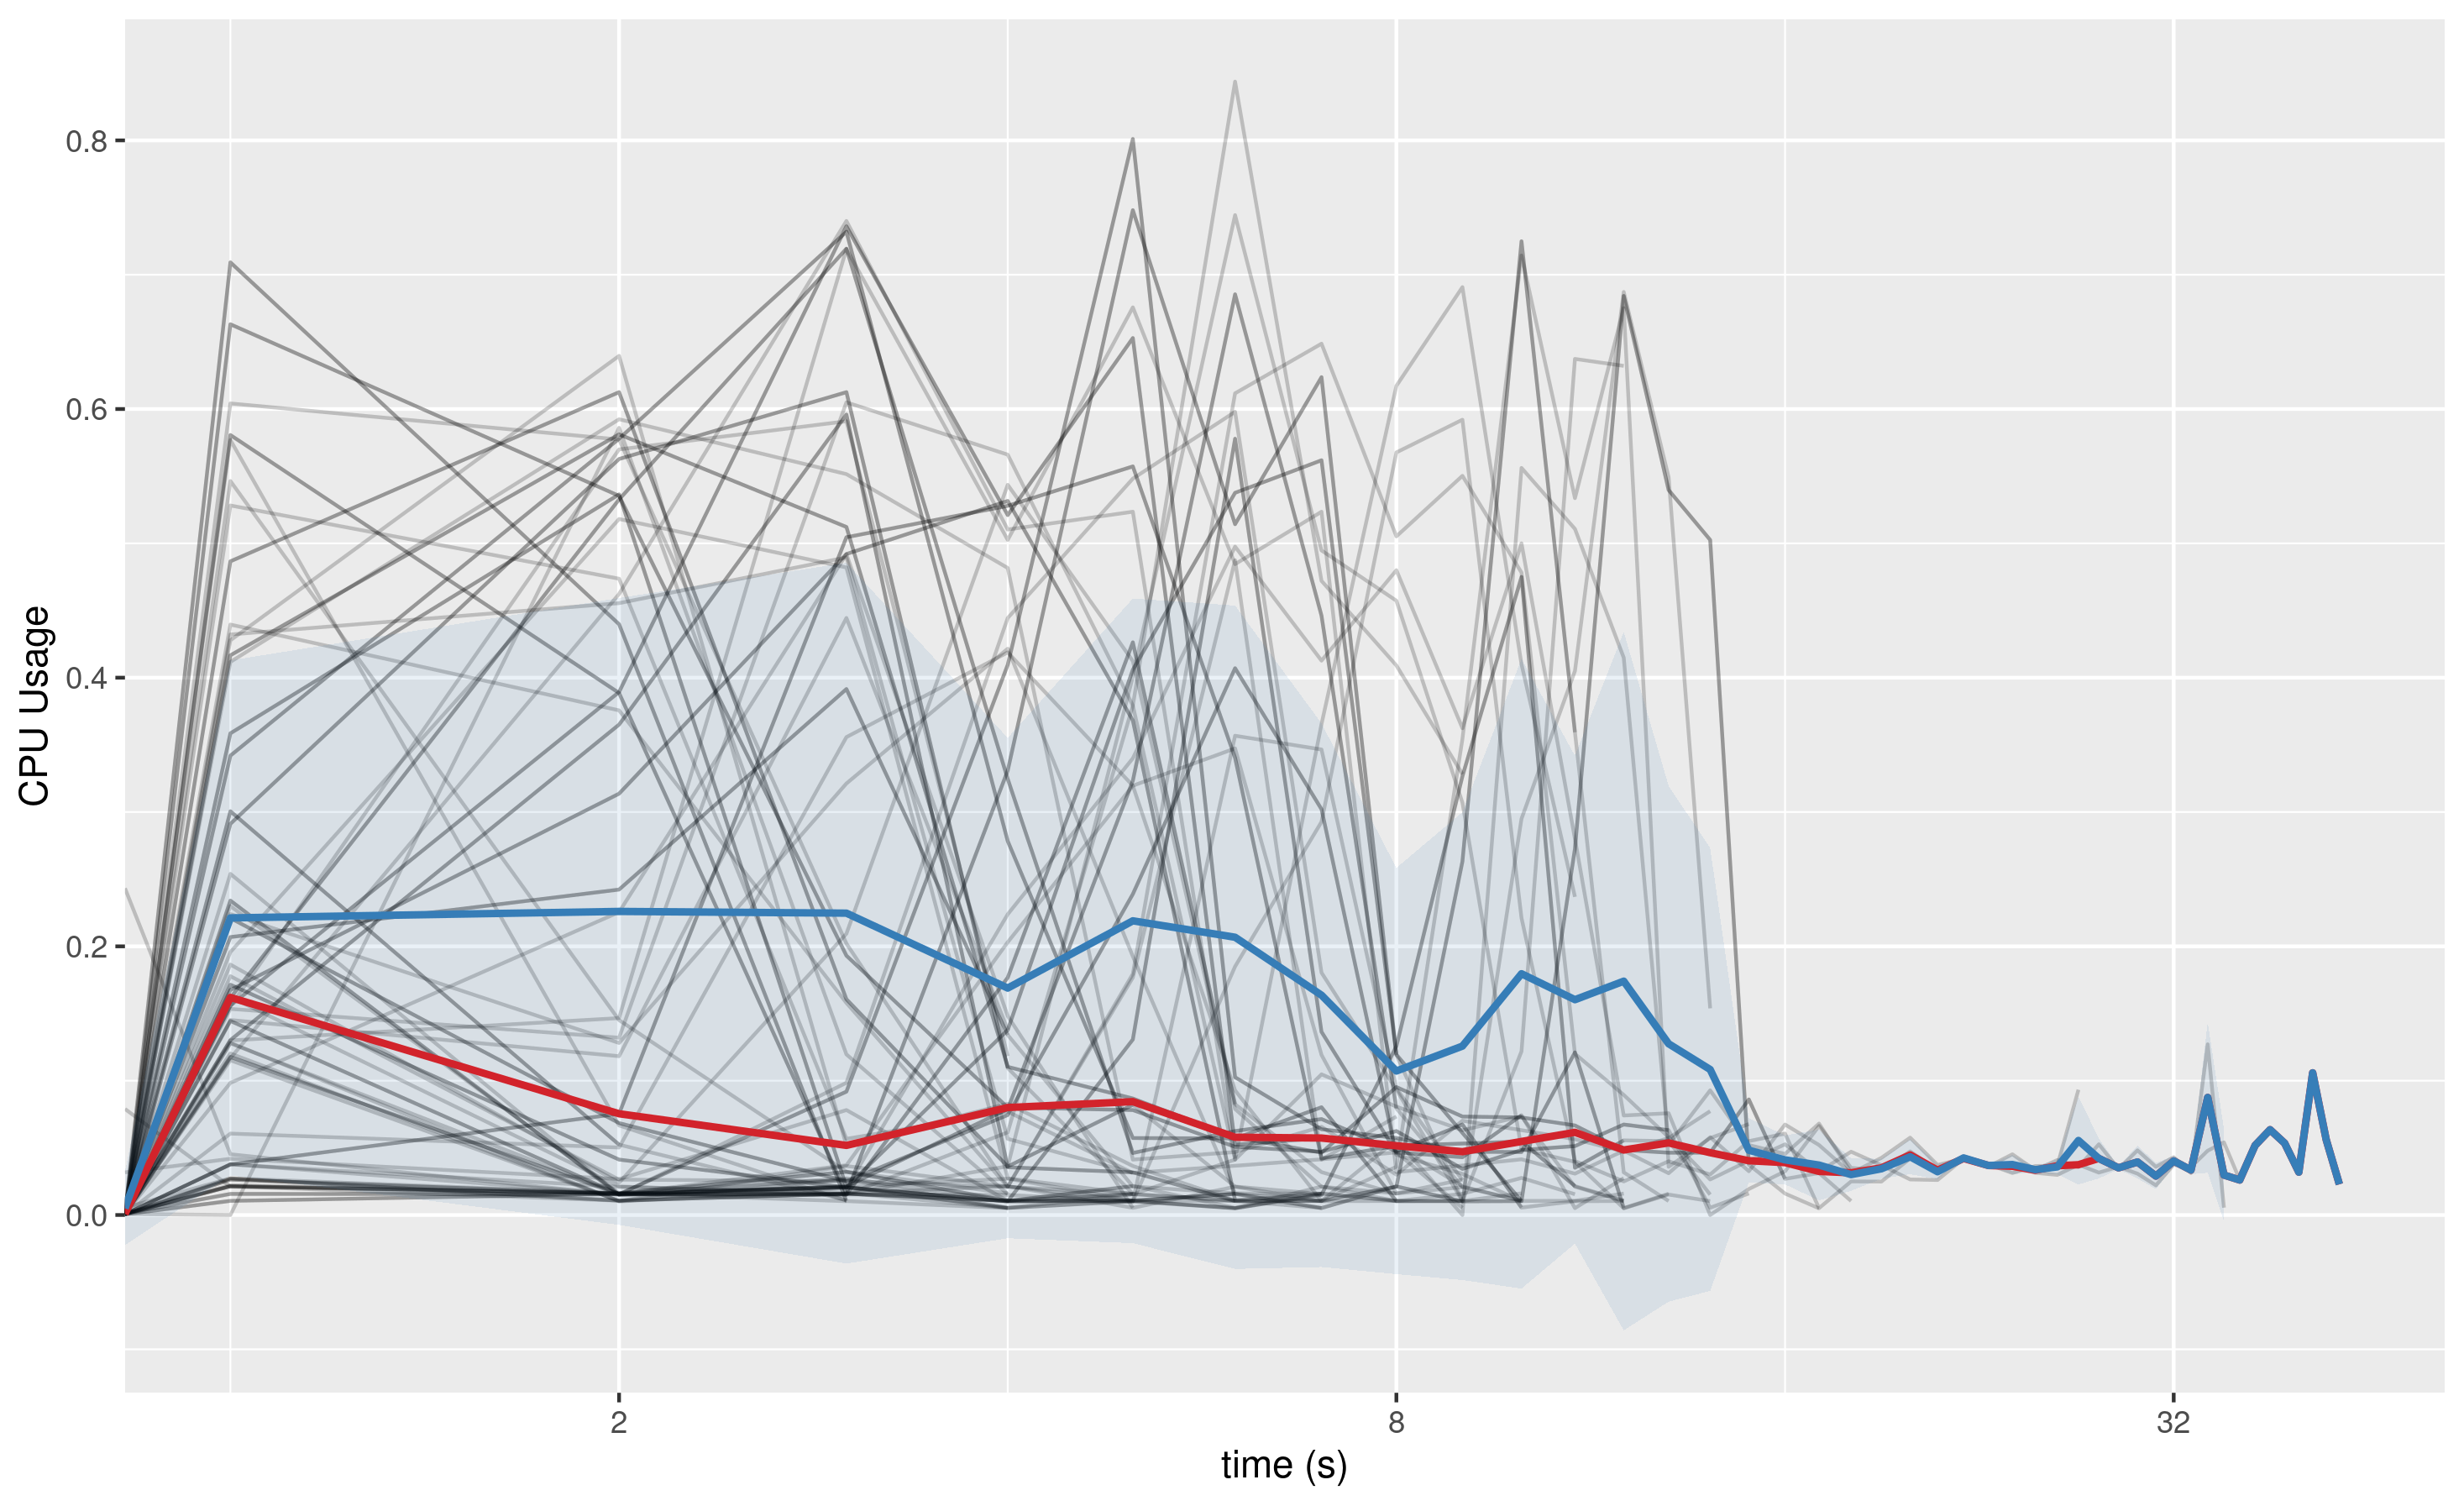
\includegraphics[width=\textwidth]{../../plots/cpu_experiment.png}
\end{frame}

\begin{frame}{Evaluation: Memory (\SI{64}{\mebi\byte})}
  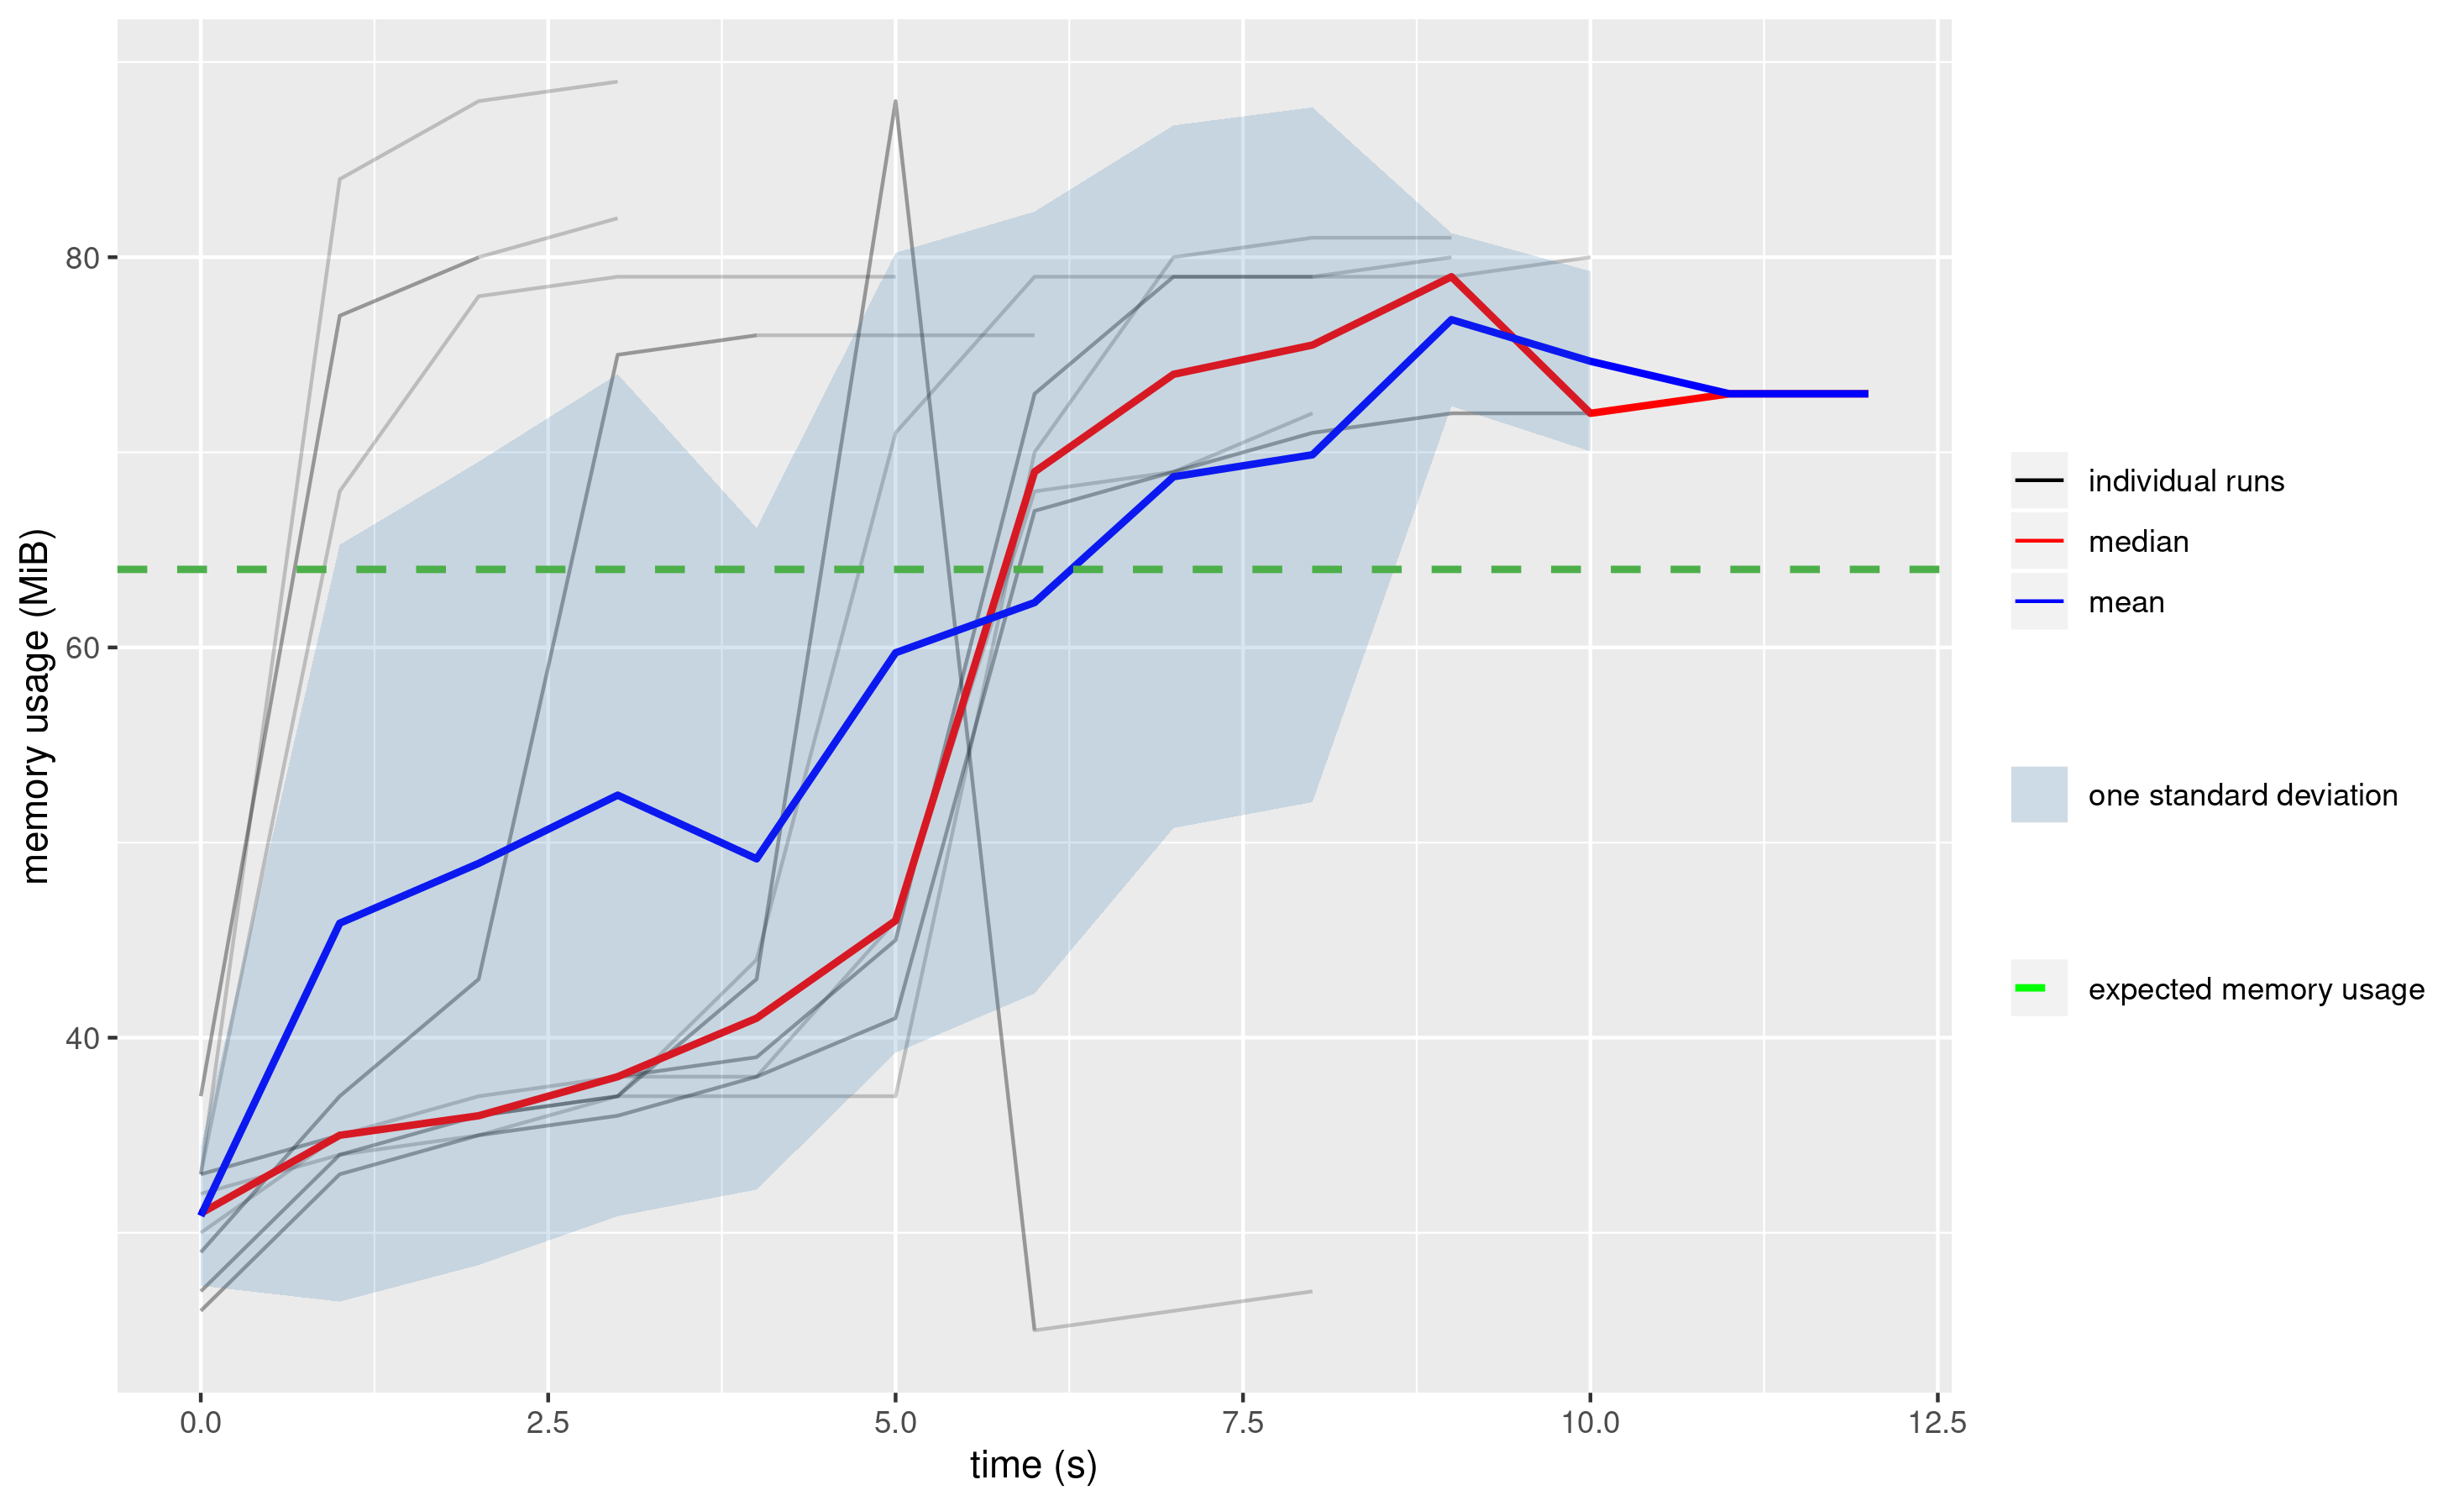
\includegraphics[width=\textwidth]{../../plots/heap_64.png}
\end{frame}

\begin{frame}{Evaluation: Memory (\SI{128}{\mebi\byte})}
  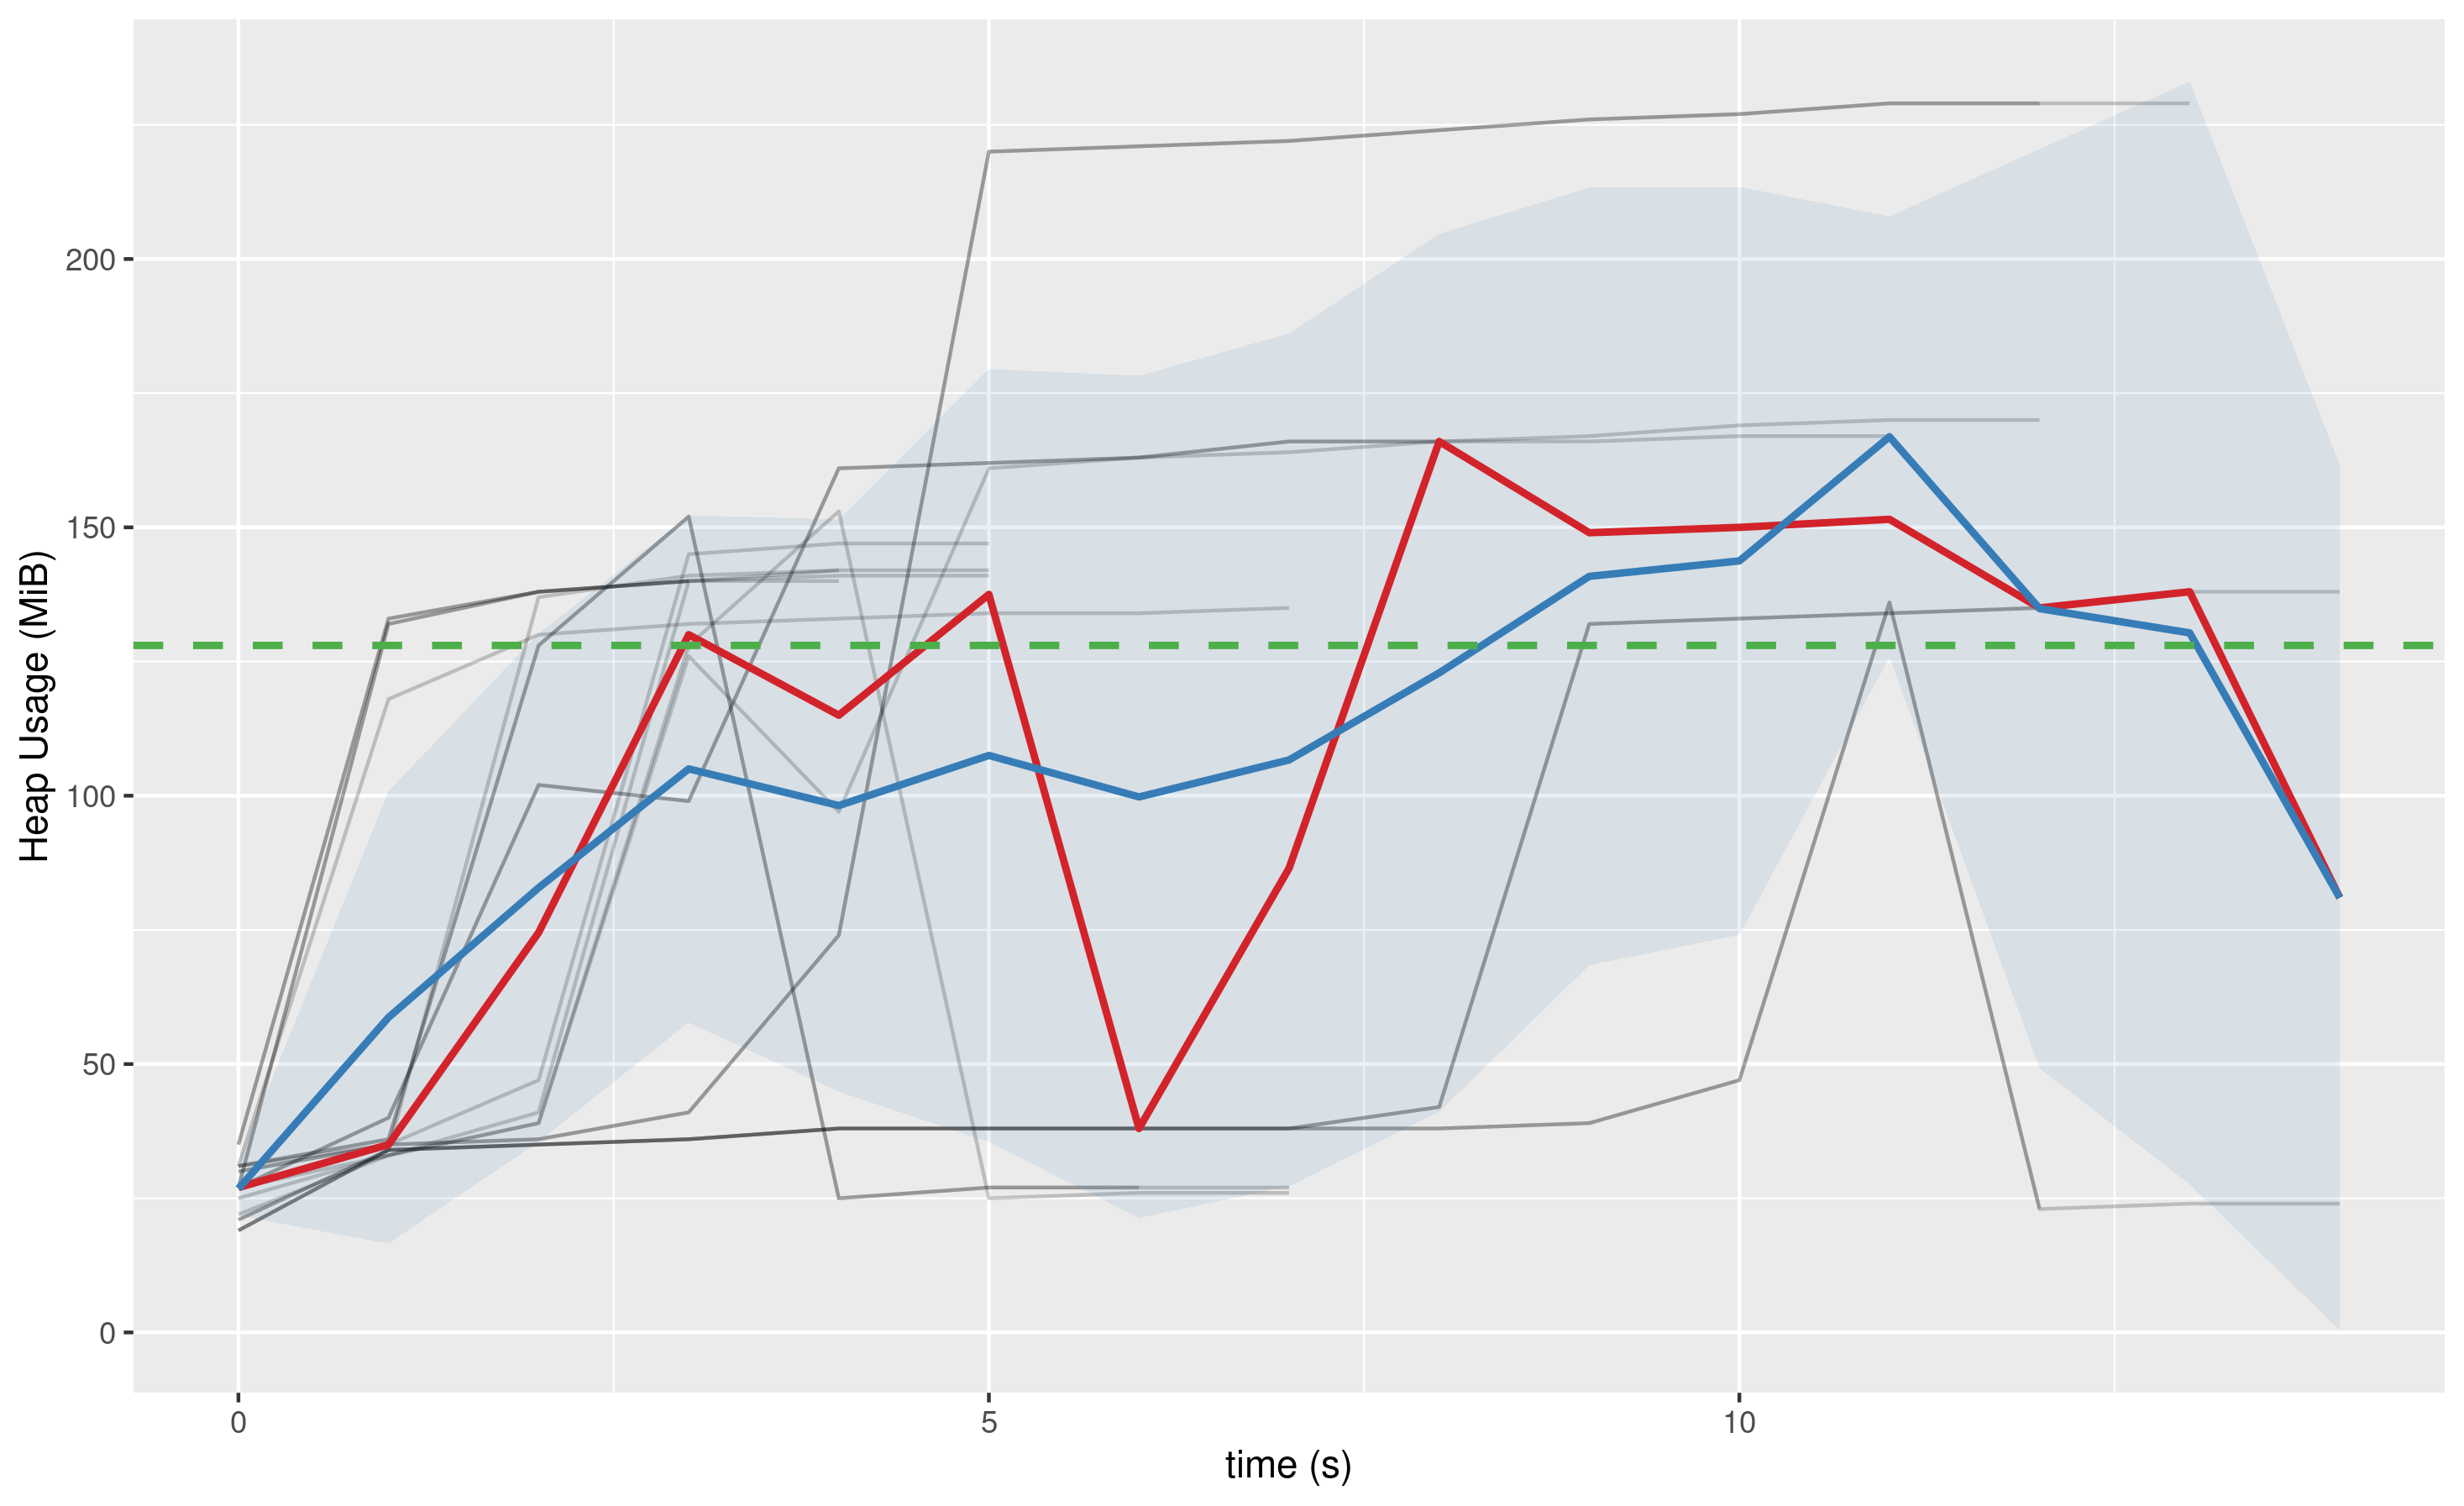
\includegraphics[width=\textwidth]{../../plots/heap_128.png}
\end{frame}

\begin{frame}{Evaluation: Memory (\SI{256}{\mebi\byte})}
  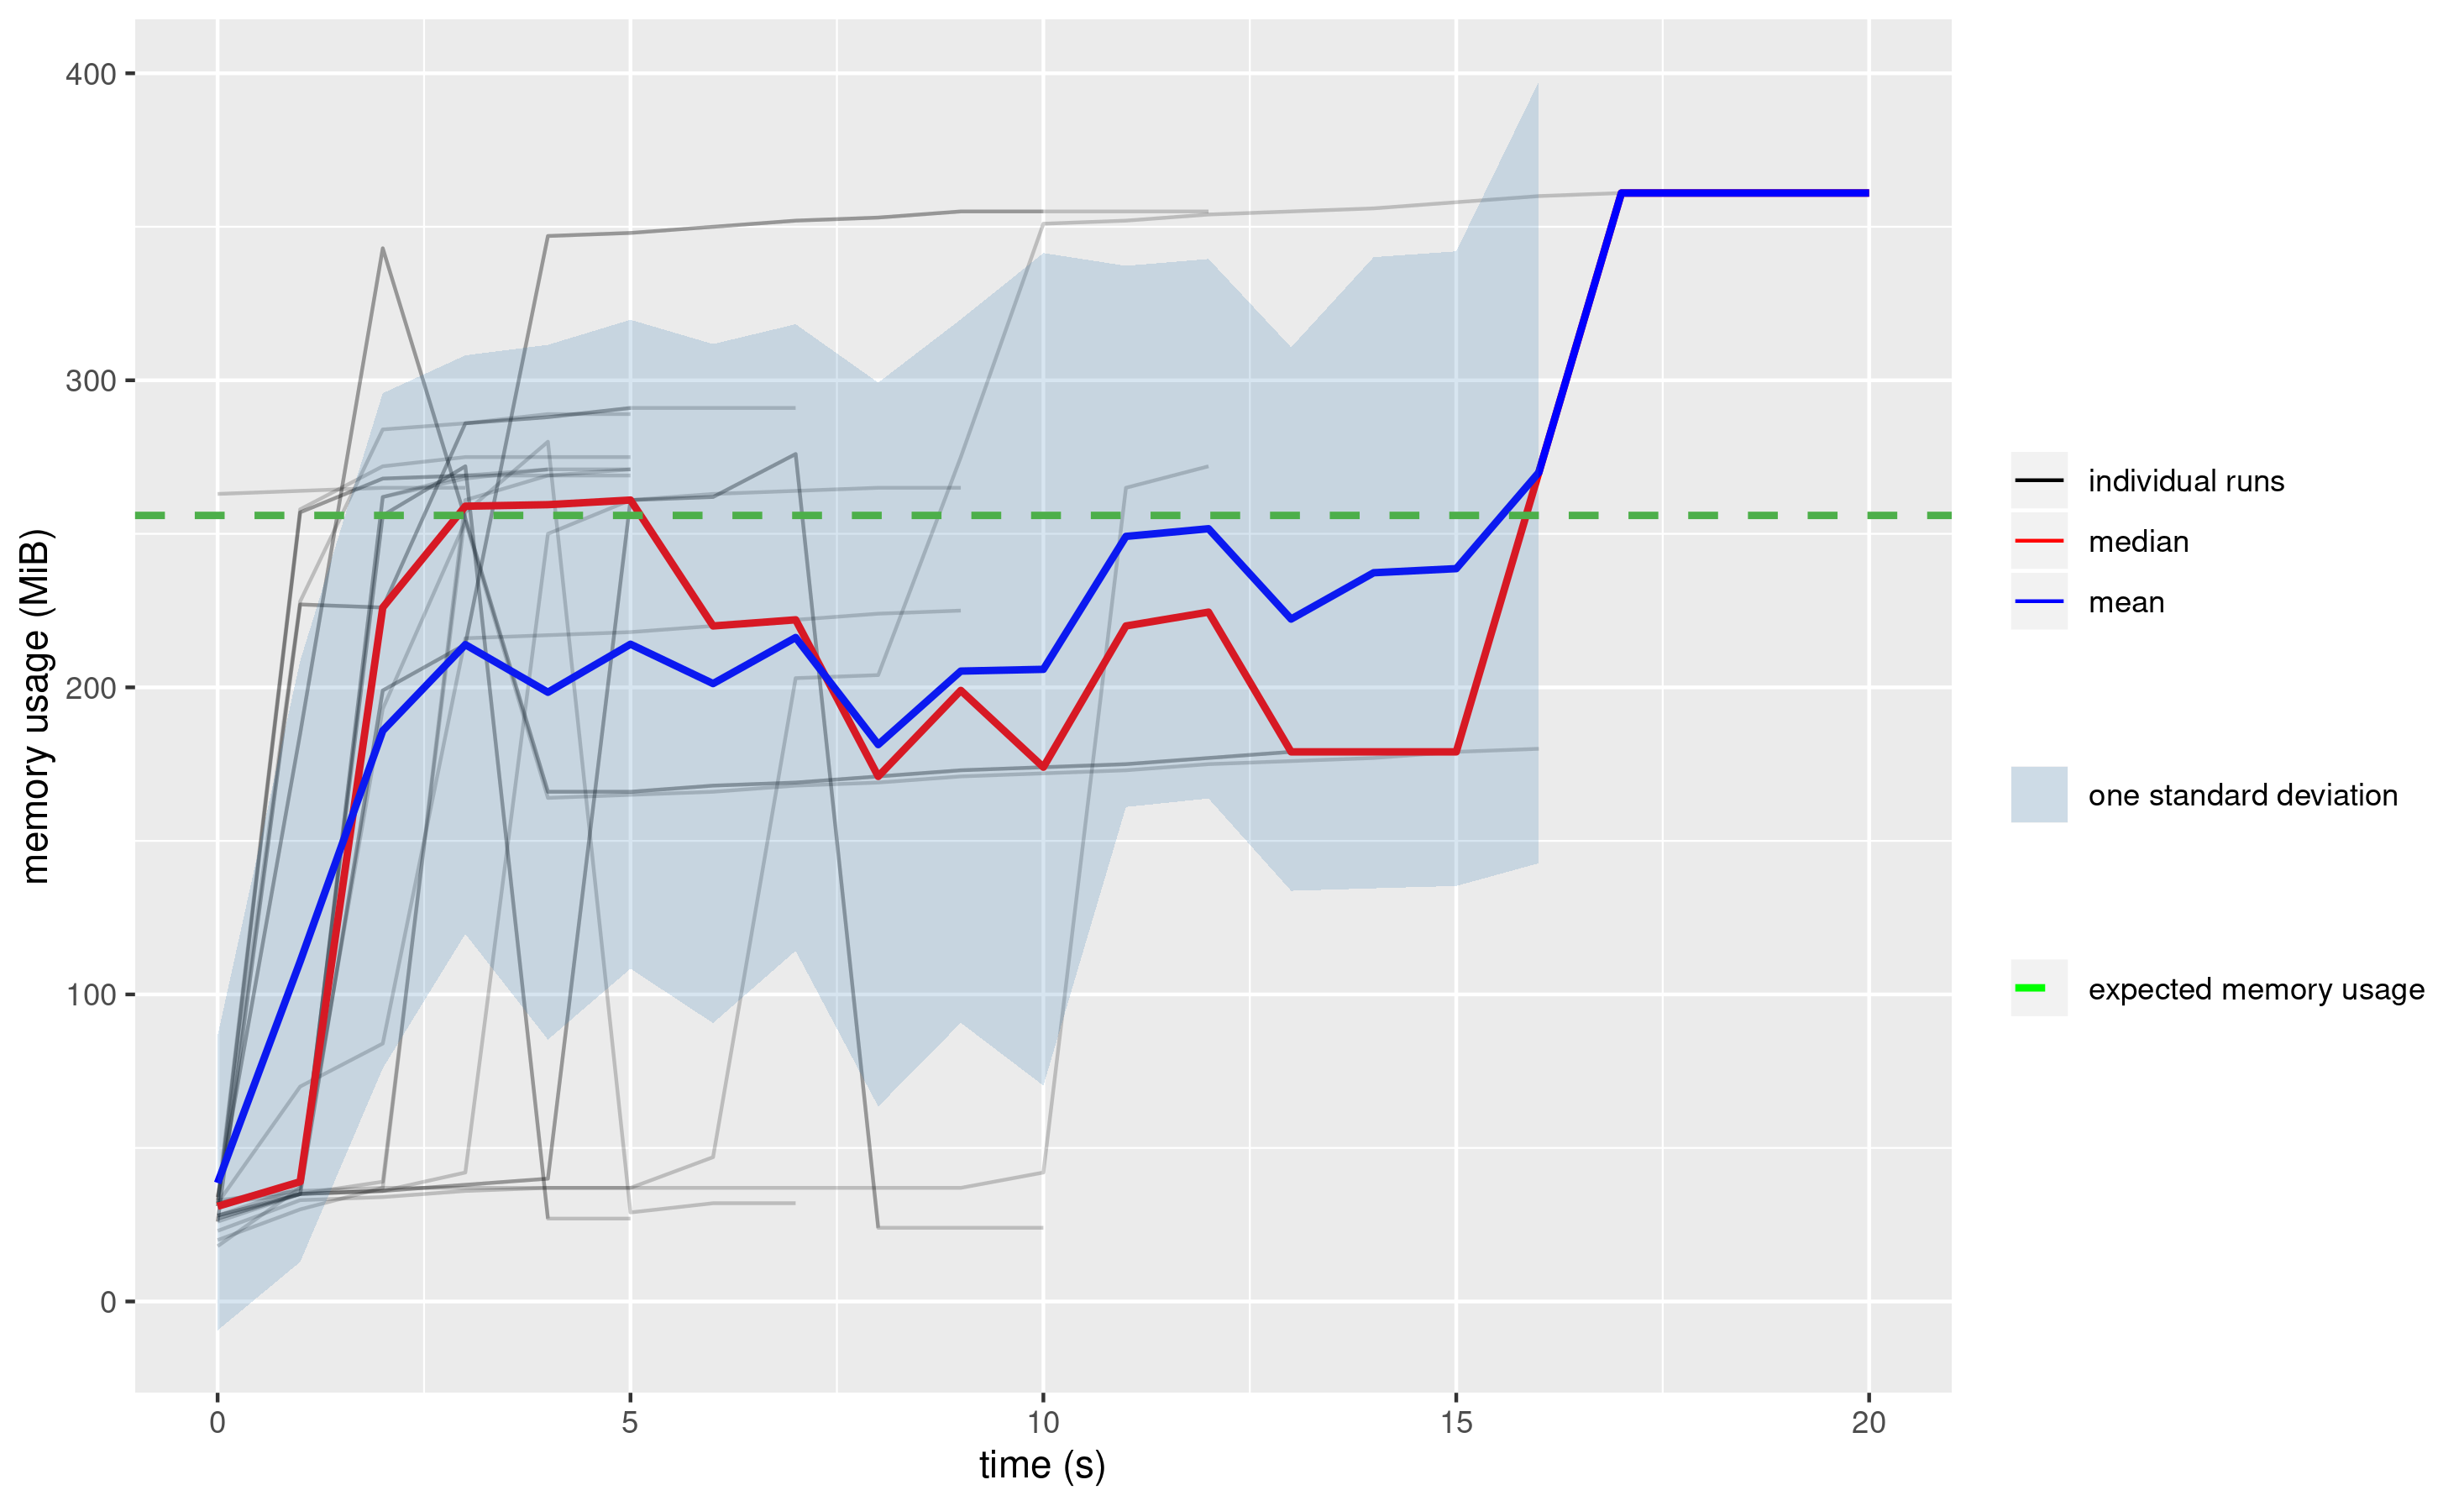
\includegraphics[width=\textwidth]{../../plots/heap_256.png}
\end{frame}

\begin{frame}{Evaluation: Memory (\SI{512}{\mebi\byte})}
  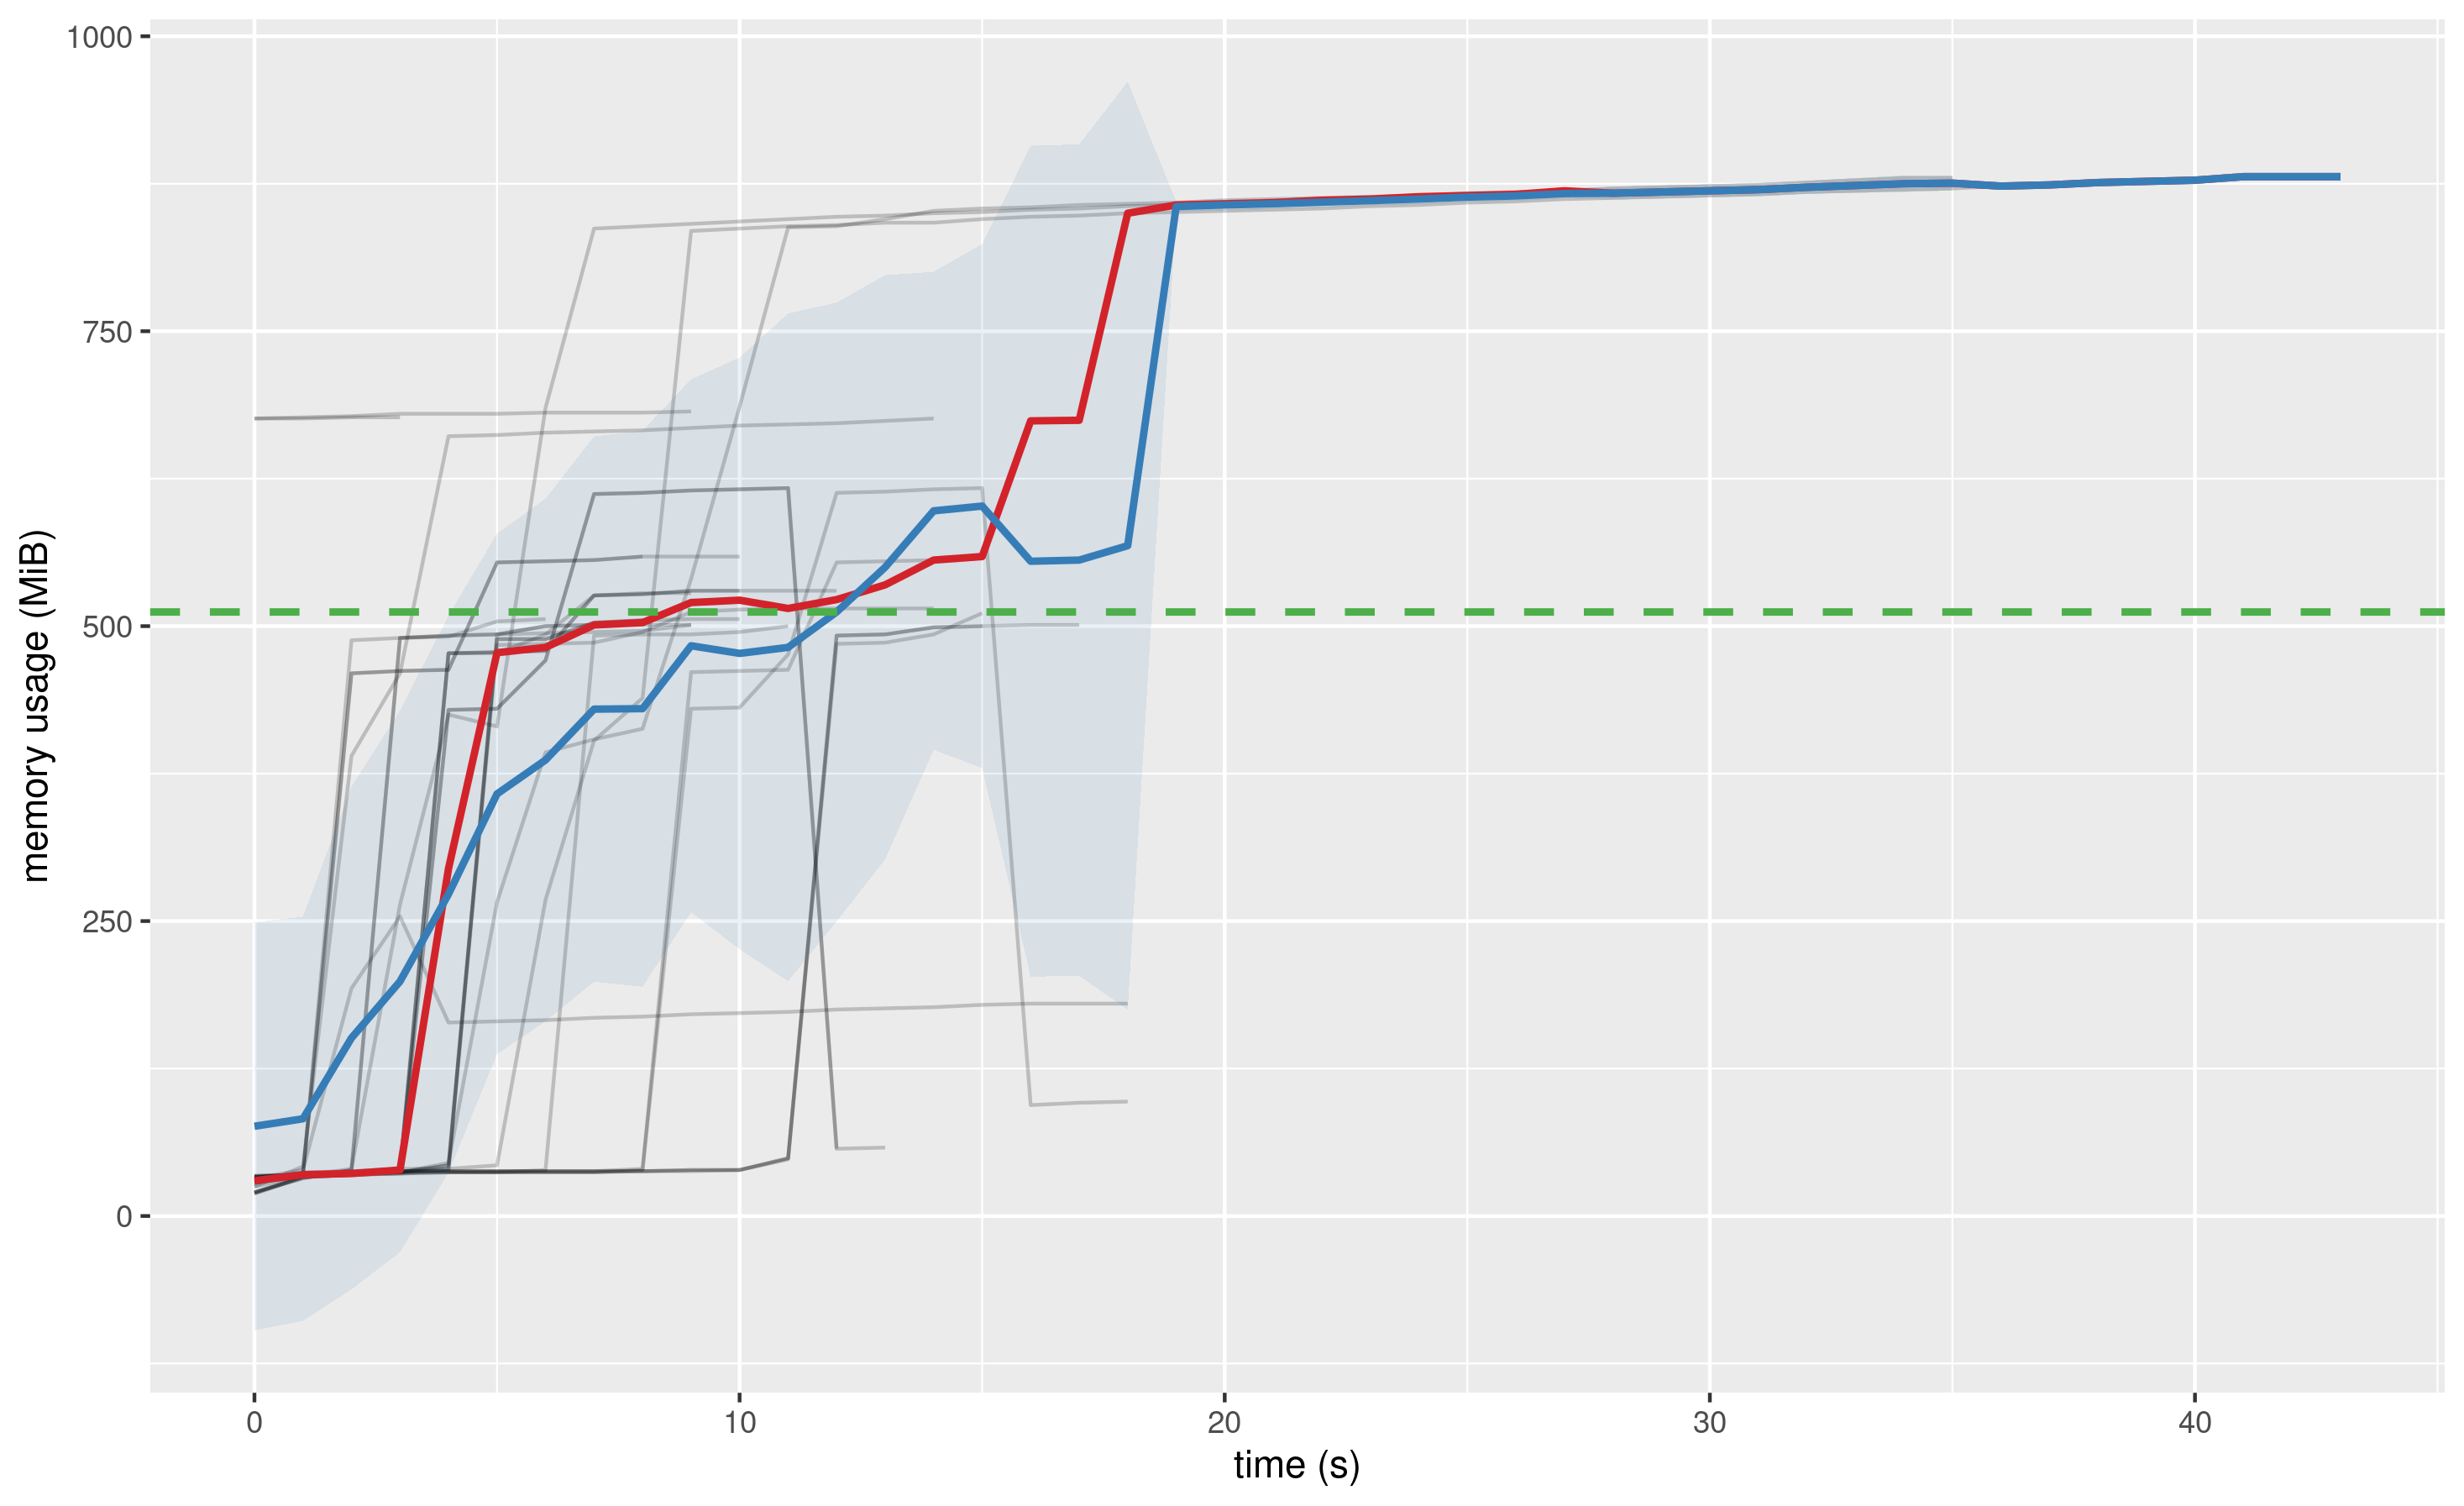
\includegraphics[width=\textwidth]{../../plots/heap_512.png}
\end{frame}

%\begin{frame}{Using Maximum Value as a Predictor}
%  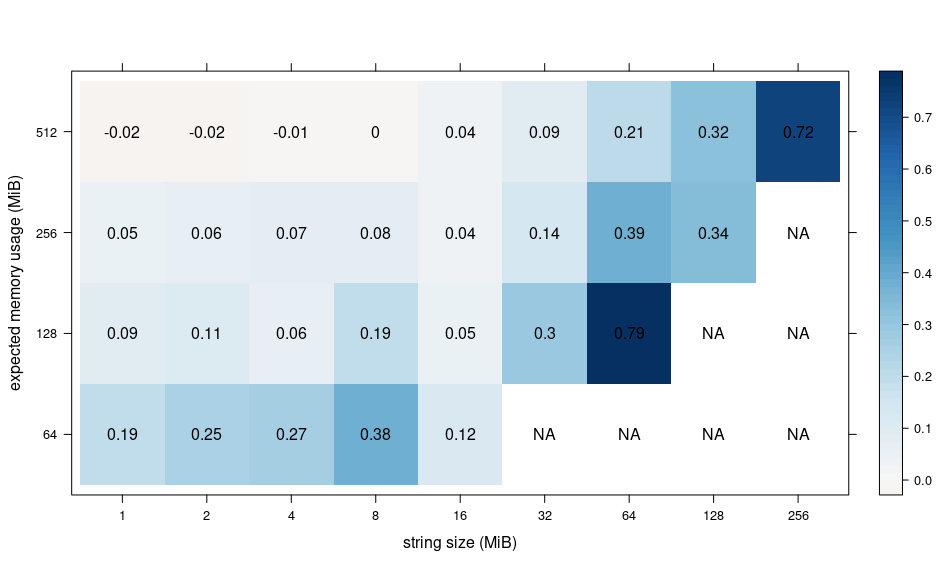
\includegraphics[width=\textwidth]{../../plots/relative_median_errors.png}
%\end{frame}

\begin{frame}{Future Work}
  \begin{itemize}
  \item Input/output simulation
  \item Complex usage patterns
  \item Automatically answering the question:
    \begin{itemize}
    \item does this experiment show that the application could benefit from more
      resources?
    \end{itemize}
  \item Complex component topologies
  \item More performance metrics (e.g. end-to-end latency)
    \begin{itemize}
    \item and example applications
    \end{itemize}
  \end{itemize}
  \pause
  \vfill
  \centering
  \large
  \emph{Thank You!}
\end{frame}

% TODO: mention:
% problem: predictions are not accurate: neither theory nor linear models
% provide good predictions. More complicated models bring their own problems.
% I'm going to try some kind of weighted/biased approach that prioritises
% fitting smaller data.

\end{document}